\begin{figure}[t]
  \centering
  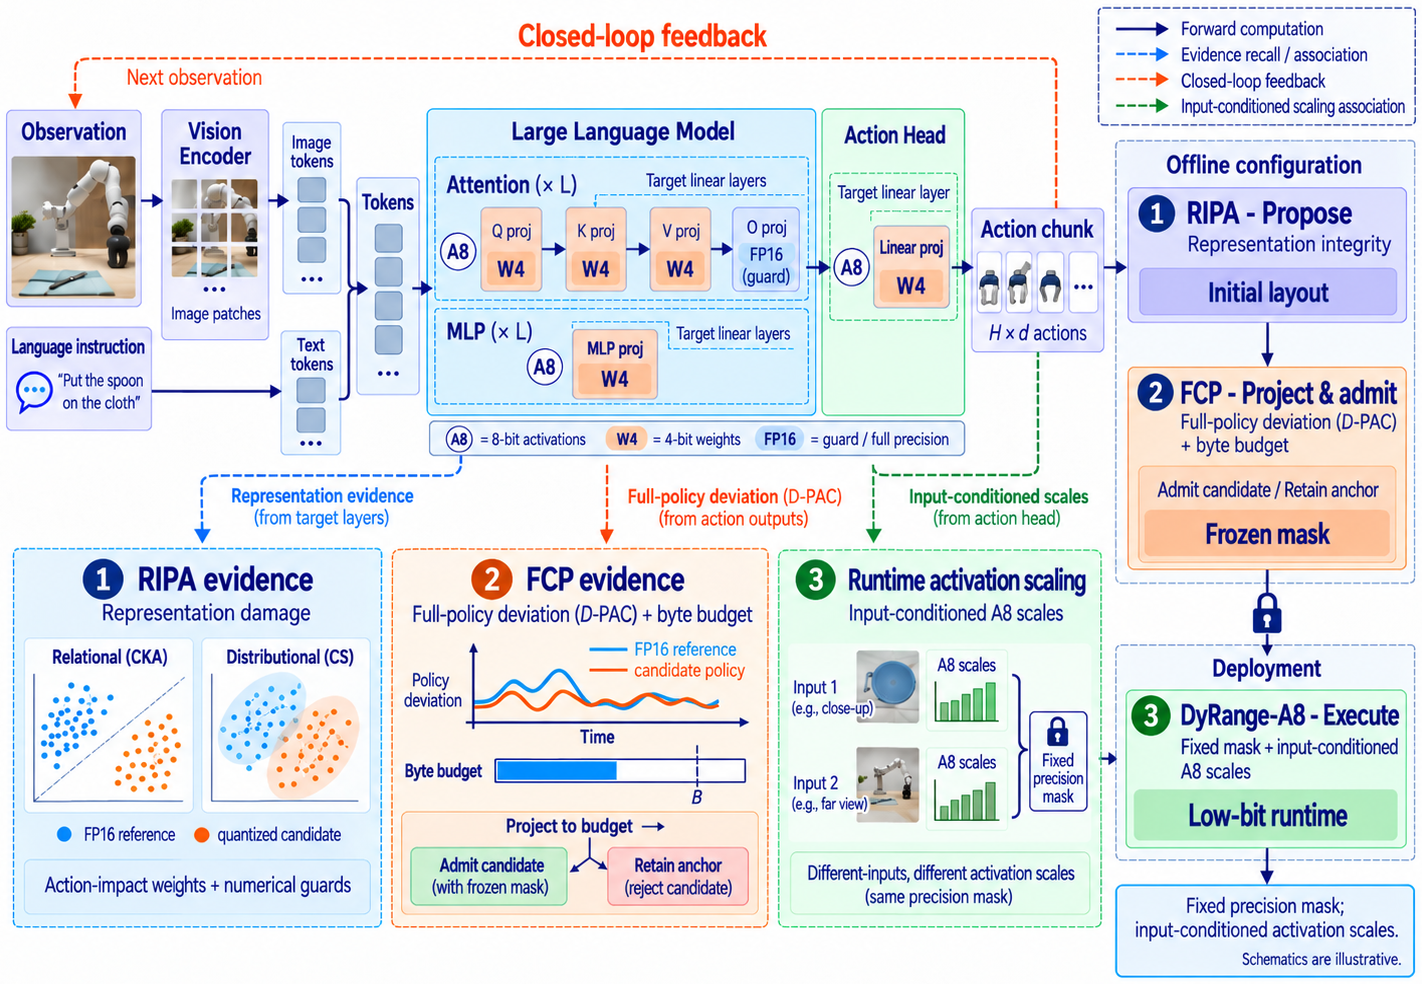
\includegraphics[width=0.86\textwidth]{figures/dypac_main_architecture_gpt_image_2_v7.png}
  \caption{Three-stage representation-to-action quantization. RIPA compares relational and distributional damage and produces a guarded layout. FCP evaluates paired action sequences with D-PAC and component conditions, projects to the budget, and accepts an eligible candidate or retains the anchor. DyRange-A8 keeps the deployment mask fixed while adapting activation scales to each input. The diagram is schematic rather than a measured result.}
  \label{fig:pipeline}
\end{figure}
